\documentclass[oneside,a4paper]{article}
\usepackage{amsmath}
\usepackage{amssymb}
\usepackage[style=ieee]{biblatex}
\addbibresource{references.bib}
\usepackage{graphicx}
\usepackage{booktabs}
\usepackage{multirow}
\usepackage{lscape}
\usepackage{longtable}
\usepackage{textcomp}
\usepackage[margin=1in]{geometry}
\usepackage{float}
% % Times new roman font
% \usepackage{mathptmx}
%% Arial font
%\usepackage{helvet}
%\renewcommand{\familydefault}{\sfdefault}
\usepackage{hyperref}
\usepackage[all]{hypcap}
\title{Detecting abnormalities on chest X-rays using deep neural networks}
\author{
  Swaroop Kumar M L\\
  % Department of Studies in Computer Science\\
  % University of Mysore
}
\date{}
\begin{document}
\twocolumn[
\begin{@twocolumnfalse}
\maketitle
\renewcommand\abstractname{\large{\textbf{Abstract}}}
\begin{abstract}
  Diseases like pneumonia and tuberculosis are leading causes of
  death world-wide and chest radiography can be an important diagnostic aid since it is fast, affordable and highly sensitive. Moreover, automated detection of abnormalities on the chest X-ray can aid the radiologist by being part of a larger system integrated into her workflow, and help in triaging and active case finding. Inspired by previous work, we develop algorithms that can detect abnormalities on the x-ray and explain these detections by generating heatmaps pointing out areas of the image that most
  influenced it. We establish baselines, benchmark against previous work and
  show that a) transfer-learning from a large non-TB dataset dramatically
  improves TB detection, b) models in the domain show inferior performance
  on external data from a different hospital system, c) mixup, a recently proposed data augmentation technique, and progressive resizing, improve performance and generalization, d) models trained to detect tuberculosis, especially those pre-trained on a large non-TB dataset, tend to overdiagnose TB, and e) saliency maps for most abnormalities show high activations at image corners around regions of the image containing shadows of metal tokens. We achieve performance competitive with previous work in
  detecting pneumonia-like and other abnormalities on the NIH chestX-ray14
  dataset and in detecting tuberculosis on the Shenzhen hospital dataset. We compare performance with and without lung-segmentation, look for potential sources of bias by training networks to identify gender, age and view-position from images alone, test
  our baseline for variable performance with respect to these, and evaluate
  our models on viral and bacterial pneumonia separately.\\
\end{abstract}
\end{@twocolumnfalse}
]

\section{Introduction}

Pneumonia and tuberculosis are leading causes of death worldwide. According to
the world health organization, pneumonia disproportionately affects children,
accounting for 16\% of all deaths of children under the age of 5
years\cite{who_pneumonia}. Tuberculosis is more prevalent in countries where
many people live in absolute poverty\cite{tb_poverty} with limited access to
healthcare and in 2017 alone, caused 1.6
million preventable deaths\cite{who_tb}.\\

The global End TB strategy aims for a 95\% reduction in deaths due to TB by 2035 compared with 2015. Similarly, the National Strategic Plan (NSP) 2017-2025 sets
out to achieve a rapid decline in deaths due to TB and emphasizes the importance
of active case finding, that is, detection of TB cases early by seeking out
people in targeted groups and scaling up cheap and high sensitivity TB
diagnostic tests. The NSP has recommended three tests: sputum smear microscopy,
chest x-ray and the new CB-NAAT\footnote{CB-NAAT or Cartridge Based Nucleic Acid
  Amplification Test is a molecular test and is
  known as GeneXpert outside India} test.\\

Conventionally, patients are screened for TB or pneumonia related symptoms,
sputum examinations are recommended for those with positive symptoms, and chest
x-rays are recommended for those who test negative in the sputum examination.\\

With automated detection, x-ray tests have the potential to be faster and
significantly more affordable. They can be massively scaled up and used
\begin{enumerate}
\item{For active case finding in high-risk populations, for example, with mobile
    x-ray vans\cite{modi_suresh_2019}}
\item{As an initial screening test before or along with other tests such as a
    sputum examination}
\item{To aid a radiologist in her workflow by sorting her queue based on
    severity, suggesting areas to consider in an image, providing a second
    opinion, etc.}
\end{enumerate}

\section{Previous work}
In \cite{Wang2017}, Wang et al. collect chest x-ray images and their associated
reports from the PAC system of the National Institutes of Health and mine labels
from the reports algorithmically. Previous work has explored methods to improve classification performance. In
\cite{Guan2018,Tang2018,Wang2018b,Pesce2017}, the authors use attention-guided
learning to allow a network to concentrate on abnormal regions of the image.
\cite{Tang2018} also uses curriculum learning and presents images in increasing
order of difficulty. However, \cite{Cai2018} uses attention to hide the most
salient regions, allowing the network to pay attention to other areas.
\cite{Yao,Wang2018b} seek to exploit correlations between abnormalities,
\cite{Yao} by using an LSTM and \cite{Wang2018b} by extracting saliency maps at
an intermediate layer and providing these as input to subsequent layers.\\

There has also been work on improving localization by combining feature maps
from multiple layers of the network \cite{Yao2018a,Sedai2018}. \cite{Sedai2018}
learns a set of \emph{layer relevance weights} for each class, and
\cite{Yao2018a} applies a DenseNet per resolution orthogonal to a standard
ResNet followed by upsampling and concatenation.\\

In \cite{Rajpurkar2018}, Rajpurkar et al. train a variant of DenseNet on the NIH chestX-ray14 dataset relabeled using an ensemble of classifiers and report
super-human performance for several abnormalities, comparing board-certified
radiologists and the algorithm on a test set labeled by consensus of three
cardiothoracic subspeciality radiologists.\\

For TB detection, previous work such as \cite{Jaeger2014,Lopes2017,Vajda2018}
have explored various feature extraction techniques, feature selection
strategies and classifiers such as logistic regression and SVM.
\cite{Hwang2016,Islam2017,Haloi2018a,Liu2018} train deep convolutional neural
networks and ensemble these. These methods have also explored the usefulness of
segmentation of chest regions. Due to the lack of large publicly available
datasets, work in this domain, especially the application of deep learning
methods, has been limited. Moreover, results are less relevant to clinical
practice as models trained on small two-class datasets are prone to over-diagnose.\\

\section{Datasets}
We use the NIH ChestX-ray14 dataset\cite{Wang2017} and the Shenzhen hospital
tuberculosis dataset\cite{jaeger2014two} to train models to detect pneumonia and other abnormalitites, and tuberculosis respectively. We then use two external
datasets, the Guangzhou medical center pediatric pneumonia
dataset\cite{kermany2018identifying} and the Montgomery county tuberculosis
dataset\cite{jaeger2014two} as \emph{external} datasets to test the ability of
these models to generalize to other hospital systems.\\

We split the NIH CXR-14 into train, validation and test sets roughly in the ratio
70:10:20. We make sure that there is no patient overlap, that is, all images of
a patient are in the same subset since patient overlap may lead to overfitting. We use the standard test set of the Guangzhou dataset and split the rest of the dataset into train and
validation sets in the ratio 80:20. However, when using this as an external dataset, we use the entire dataset. Considering the small size of the Shenzhen and Montgomery datasets, we create 9 folds and
report average and standard deviation of metrics. Each fold contains all the
images split into train, validation and test sets in the ratio 70:10:20. However, when using the Montgomery dataset as an
external dataset, we ignore these folds and test on the
entire dataset.


\section{Model}
We replace the final fully connected layer of 121-layer dense convolutional
neural network with one that has either 14 outputs (for the NIH CXR-14 dataset)
or 2 outputs (for all other datasets) after which we apply a sigmoid
non-linearity. The fully convolutional backbone of the network results in $k$
$w$ x $h$ feature maps and is followed by a global-average-pooling layer where
the $k$ feature maps are averaged along the width and height to form a $k$
dimensional vector. This makes the network independent of input image size and
allows us to use the
progressive-resizing method. The network's connectivity pattern improves the flow of information and
gradients and has fewer parameters, making it possible to train very deep
networks. The architecture of the model, specifically the fact that the fully
convolutional part of the network is followed by a single fully connected layer,
forces the model to learn to localize abnormalities given only weak labels (presence or absence of an abnormality).

\begin{figure*}[]
  \centering 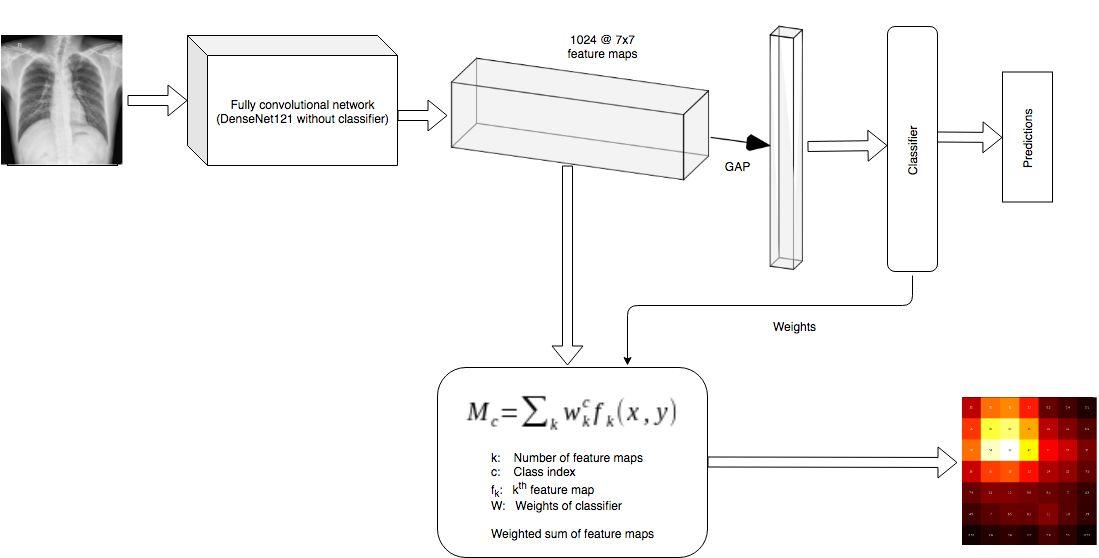
\includegraphics[width=\textwidth]{images/arch}
  \caption{Basic architecture of the model}
  \label{architecture}
\end{figure*}

\section{Training and inference}
We use the Adam optimization algorithm and start the training with an initial
learning rate a factor of 10 smaller than the learning rate at which the
training loss begins to increase, when the learning rate is increased linearly
(using a learning rate finder). We divide the learning rate by 10 if the
validation loss plateaus (does not decrease over 5 iterations), and stop
training when the validation loss has stopped decreasing. When using k-fold
cross validation, we train $k$ different networks on each of the $k$ folds and
report average and standard deviation
of performance.\\

At the multi-class multi-label classification task (for the NIH CXR-14 dataset),
we merge the train and validation sets after training and use it to compute
optimal thresholds for each abnormality by optimizing for the class-specific
F1-score. Although it is possible to compute optimal thresholds for the
classification task since we have ground truth labels, it is not possible to do
so for the localization task since
we only have weak labels and not precise locations. At binary classification tasks, since the network has two output nodes, we do
not compute thresholds but simply consider as the proper output the class whose
corresponding output node has higher activation.

\section{Explainability}
Deep neural networks have outperformed previous methods in several domains.
However, they remain black-boxes with millions of parameters, leading to a lack
of trust and limiting their use in routine clinical practice.\\

Several methods
have been proposed to make these models more interpretable, broadly falling into
two categories: a) methods that create a proxy model which behaves similarly to the original
model, but is simpler and easier to understand, which include methods like
LIME\cite{ribeiro2016should} and SHAP\cite{NIPS2017_7062}which are model-independent but tend to be very slow. and b) methods that generate a saliency map which highlights a small portion of
the input which is most relevant, in a single forward and backward pass
through the networkwhich include methods like LRP\cite{bach2015pixel},
DeepLIFT\cite{shrikumar2017learning}, CAM\cite{zhou2016learning} and
    Grad-CAM\cite{selvaraju2017grad}.\\

We use the CAM method. To compute explanations, we save the feature maps resulting from the final
convolutional layer during a forward pass and perform a weighted sum of these
feature maps using the weights of the final fully-connected layer between
each of the feature maps and the desired output node, as follows.\\

If $f_i$ is the $i^{th}$ feature map and $w^j _i$ is the weight between the
$i^{th}$ input node and the $j^{th}$ output node in the fully-connected layer,
the saliency map for the $j^{th}$ class $M_j$ is
\begin{equation}
  M_j = \sum _i \, w^j _i \, f_i
\end{equation}
$M_j$ is a $w$ x $h$ saliency map which we interpolate to the size of the input
image and visualize as a heatmap.\\

We use a region-growing algorithm to determine bounding boxes given a saliency
map. Specifically, we first threshold the saliency map and using the maximum
element as a seed point, grow a region around it, including all non-zero
neighbours, and repeat the same until all non-zero elements are included in a
region, each time choosing as seed the maximum element not included a region.
For each region, we determine a bounding box as the smallest rectangle which
encloses the entire region (for example, see \ref{cam_bbox_examples}).

\begin{figure}
  \centering
  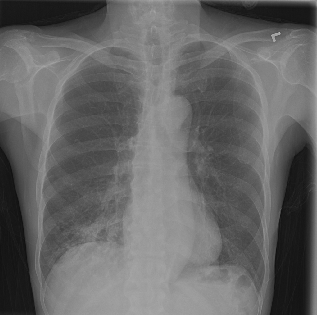
\includegraphics[width=0.2\textwidth]{images/preds/pneumonia}\hspace{0.01\textwidth}%
  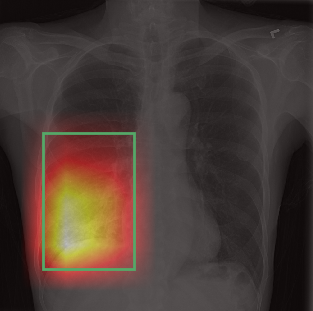
\includegraphics[width=0.2\textwidth]{images/preds/pneumonia_cam}\\[0.01\textwidth]
  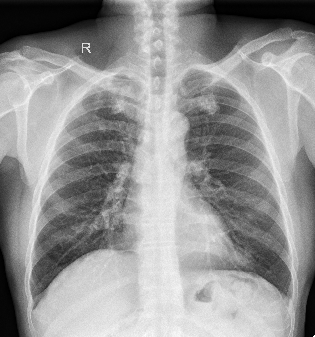
\includegraphics[width=0.2\textwidth]{images/preds/TB2}\hspace{0.01\textwidth}%
  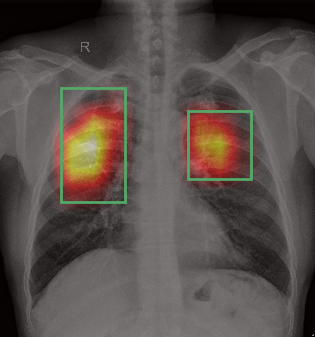
\includegraphics[width=0.2\textwidth]{images/preds/TB2_cam}\\[0.01\textwidth]
  \caption{Examples of saliency maps with corresponding bounding boxes drawn.
    The first column shows original x-ray images and the second row shows
    saliency map and bounding boxes overlaid on the image. Row 1: Pneumonia. Row
    2: Tuberculosis.}
  \label{cam_bbox_examples}
\end{figure}

\section{Generalizability}
A test set is considered representative of data that will be encountered in the
external world and is used exclusively to evaluate a model. However, true
generalization to new datasets may be lower than expected. Two datasets may have different distributions. In the context of
biomedical imaging, datasets may be collected from different hospital
systems and machines. For example, in \cite{zech2018variable}, Zech et al.
show that models trained on data from one hospital system showed inferior
performance on data from others. The dataset used to train a model may have confounding variables that do
not exist in other datasets. For example, in \cite{zech2018variable}, Zech
et al. also show that CNNs were able to directly detect the hospital system
and department within a hospital system from a chest radiograph where
saliency maps showed high activation in image corners. We observed the same
phenomenon in networks that were trained to detect abnormalities (figure \ref{avg_saliency_maps} shows average saliency maps or explanations weighted by predicted probability). Since
different departments and machines within a hospital system have different
prevalence of a disease, the model may leverage these spurious correlations
and fail to generalize. \\

\begin{figure}[]
  % \fbox{
  % \begin{minipage}{\textwidth}
  \centering
  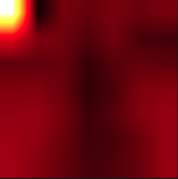
\includegraphics[width=0.28\textwidth]{images/heatmap_224_da}\\[0.01\textwidth]
  \caption{Average saliency maps for \emph{pneumonia} of the baseline model trained on the NIH CXR-14 dataset.}
  % \end{minipage}
  % }
  \label{avg_saliency_maps}
\end{figure}

We evaluate the ability of our baselines to generalize to other hospital
systems. At the problem of pneumonia detection, we train on the NIH CXR-14
dataset and test on both the internal test set and the external Guangzhou
dataset, a pediatric pneumonia dataset from a different hospital system.
At the problem of tuberculosis detection, we train on the Shenzhen tuberculosis
and and test on both the internal test set and the external Montgomery
tuberculosis
dataset from a different hospital system.\\

We find that the baseline model trained to detect pneumonia on the NIH CXR-14
dataset performs better on the Guangzhou dataset than the internal test set but
worse that a model trained exclusively on the external dataset, and the baseline
model trained to detect tuberculosis on the Shenzhen dataset shows inferior
performace on the external dataset, but which is better than a model trained
exclusively on the external dataset.

\section{Transfer-learning}
We initialize the weights of a network with those of a similar network trained
on a large dataset of millions of natural images, ImageNet and compare this with random initialization (we use the Kaiming He initialization method\cite{he2015delving}) and show that pre-training on ImageNet significantly improves performance on
both internal and external datasets.\\

On the Shenzhen hospital tuberculosis dataset, we replace the weights
of a network with those of a similar network a) trained on ImageNet (a large
non-x-ray dataset of natural images) and b) trained on ImageNet and then on NIH
CXR-14 (a smaller non-tb x-ray
dataset), and observe that pre-training on the NIH CXR-14 dataset both improves performance
on both the internal test set and helps to close the generalization gap.

\section{Mixup}
Mixup, a recently proposed data augmentation technique \cite{Zhang2017}, has been shown to be effective at regularizing models and combating label
noise. Instead of using raw
images, we feed the model a linear combination of two images not necessarily
from the same class. If $I_1$ and $I_2$ are two images, we feed the network a
linear combination $M = t \cdot{}I_1 + (1 - t) \cdot{}I_2$ where $t$ is drawn
from a beta distribution parameterized by some $\alpha$. The expected output for
$M$ is $ t \cdot{} y_1 + (1 - t) \cdot{} y_2$ where $y_1$ and $y_2$ are the
targets for $I_1$
and $I_2$ respectively. Mixup improved performance on both the NIH CXR-14 dataset and the Shenzhen
tuberculosis dataset. It also improved generalization to external datasets.


\section{Progressive resizing}
For the NIH CXR-14 dataset, we first train on 224 x 224 images until the
validation loss plateaus. We then re-train the same network on 256 x 256 images,
288 x 288 images, etc. upto 512 x 512 with a smaller learning rate and for
fewer epochs. For the Shenzhen hospital tuberculosis dataset, we first train on 224 x 224
images, until the validation loss plateaus, and retrain the same network on 448
x 448 images and then on 672 x 672 images.\\

The intuition behind progressive resizing is that first training
on lower resolution images is equivalent to pre-training and is better than
training on high resolution images from scratch. It may also make networks more
robust to scale variation and behave similar to
data augmentation preventing overfitting. We observe that progressive resizing consistently improves performance and
generalization to external datasets.

\section{Fairness}
We look for potential sources of bias such as gender, age and view-position
by a) looking at the distribution of ground truth by gender, age and view-position and variable rates of abnormalities, b) training models with architecture similar to our baseline model to predict these from images alone. We then measure variable performance of our baseline model across gender, age-group and view-position.\\

\subsection{Age}
Age follows a rougly gaussian distribution with a mean of 46.17 years and standard deviation of 16.73. On dividing patients into 10 age groups (0-9 years, 10-19 years \dots 90-99 years), abnormality rate increases with age, with a maximum rate of 57.4\% for the age group 80-89 years and a minimum rate of 38.7\% for the age group 0-9 years. \emph{No finding} is negatively correlated with age, with a PMCC of -0.07. When broken down into 3 age groups (less than 25 years, between 25 and 65 years, and greater than 65 years) and by specific abnormalities, \emph{Hernia} is 2.8 times more likely if the patient is old-aged (more than 65 years old) and \emph{Pneumonia} is 1.4 times more likely if the patient is young (less than 25 years old).\\

However, a network with a similar architecture with 3 output nodes trained to detect the age group from x-ray images predicted the most common $2^{nd}$ age group (25 to 65 years) for every image. A network with a similar architecture with a single output node trained to predict age as a continuous variable achieved a mean absolute error of 10.9 years, which is not significantly better than the mean absolute deviation of a gaussian distribution with the same mean and standard deviation as that of patient-age, 13.3, meaning that the model's predictions are not much better than a naive algorithm which predicts the mean age of 46 years for every image.\\

We evaluated our baseline for variable performance for each age group and found that the model showed similar performance (in terms of AUROC) for each.

\subsection{Gender}
The male to female ratio is approximately 1.28, with similar rates of abnormality, 53.5\% and 54.1\% for males and females respectively, and \emph{No finding} is only weakly correlated with \emph{female}, with a PMCC of 0.006.
However, when broken down by specific abnormalities, the ratio of the posterior probability of an abnormality given the gender to its prior probability shows significant variation, with \emph{Hernia} becoming 1.3 times more likely and \emph{Cardiomegaly} becoming 1.2 times more likely if the patient is female (pregnancy is a common cause of \emph{Cardiomegaly}).\\

A similar network (with the same architecture, the only difference being 2 output nodes in the final layer instead of the 14) trained to identify gender from x-ray images on this dataset acheived an accuracy of 93.8\% (AUROC of 98.9\%) on this task when trained for a single epoch. Saliency maps showed high activations at and around regions of the image containing female breasts.\\

Although this does not necessarily mean that our abnormality-detection models are biased, the two findings above show that some bias exists in the dataset and that these models are capable of exploiting these. We evaluated our baseline model for variable performance for males and females and found that the model showed similar performance (in terms of AUROC) for both genders.

\subsection{View-position}
The PA (posterioanterior) view is preferred over the AP (anterioposterior) view. However, the AP view is usually chosen over the PA view for younger children and is necessitated for very ill patients who cannot stand erect. The PA view is more common in the NIH CXR-14 dataset with 60\% of the images showing the PA view. Abnormality rate is higher for the AP view (52.8\%) compared to the PA view (41.6\%), and \emph{No finding} is positively correlated with PA with a PMCC of 0.11. When broken down by specific abnormalities, the ratio of the posterior probability of an abnormality given the view-position to its prior probability shows significant variation, with \emph{Edema} and \emph{Consolidation} becoming 2.2 times and 1.7 times more likely respectively if the x-ray image shows AP view.\\

Moreover, a network with a similar architecture with 2 output nodes trained to identify the view-position from x-ray images acheived an accuracy of 98.7\% (AUROC of 99.7\%) on this task when trained for a single epoch. Saliency maps showed high activations at and around the anterior aspect of the ribs and around shadows of tokens on x-ray that identified the machine as being a \emph{portable} machine.\\

We evaluated our baseline for variable performace for each view-position and found that the model showed similar performance (in terms of AUROC, sensitivity and specificity).

\section{Over-diagnosis}
The rate of of tuberculosis in the NIH CXR-14 dataset is unknown since
tuberculosis is not one of the labels. However, assuming a baseline rate of less
than 1\%, we observe that models trained to detect tuberculosis on the Shenzhen
hospital tuberculosis dataset tend to over-diagnose when tested on the NIH
CXR-14 dataset. The rate of over-diagnosis is especially high when models are pre-trained on the
NIH CXR-14 dataset.

\section{Viral vs bacterial pneumonia}
Images in the Guangzhou pediatric pneumonia dataset that show manifestations
of pneumonia are further categorized as \emph{Viral} and \emph{bacterial}.
Since viral and bacterial pneumonia present different levels of emergency and warrant
different courses of treatment, we evaluate our models for variable performance on these
categories to ensure that they are not biased toward one or the other type. We found that the models trained on the NIH CXR-14 dataset were better at
detecting viral pneumonia than bacterial pneumonia.

\section{Segmentation and centering}
The Montgomery dataset includes hand-annotated segmentation masks of both the left and right lungs for each image. We evaluate models trained on the Shenzhen hospital tuberculosis dataset, on the Montgmomery dataset after a) segmenting the lung regions and b) segmeting the lung regions and cropping to the smallest rectangle which encloses both the lungs. Across multiple models and trials and averaged across 9 folds, we failed to see a significant increase or decrease in performance among models trained on un-segmented images, segmented images and segmented and cropped images.

\section{Results}
For the NIH CXR-14 dataset, we achieve performance competitive with previous
work and show improvements over our baseline. See table \ref{tab:nih_previous} for
the results. Rajpurkar et al. in \cite{Rajpurkar2018a} measured human
performance in terms of AUROC for each disease, using the majority vote of 3
independent board-certified cardiothoracic specialist radiologists (average
experience 15 years) as ground truth, and measure the the performance of 6 BC
radiologists from 3 academic institutions (average experience 12 years) and 3
senior radiology residents by fitting a curve to these 9 radiologists' operating
points and calculating the area under it. We compare our models with human
radiologist performance and find that the model's performance is on average
within 2\% of that of human radiologists (see table
\ref{tab:nih_comparision} for the comparison).\\

On the Shenzhen and Montgomery datasets, we achieve performance comparable to
previous work and show improvement over our baseline. See tables
\ref{tab:shenzhen_previous} and \ref{tab:montgomery_previous} for the results.

\begin{table*}[]
  \centering
  \begin{tabular}{ll}
    \hline
    \textbf{Authors}            & \textbf{AUROC} \\ \hline
    Wang et al. (2017)          & 0.738                  \\ \hline
    Y. Shen et al.              & 0.775                  \\ \hline
    H. Wang et al. (ChestNet)   & 0.781                  \\ \hline
    P. Kumar et al.             & 0.792                  \\ \hline
    Yao et al. (2017)           & 0.803                  \\ \hline
    Y. Tang et al.              & 0.805                  \\ \hline
    S. Guendel et al.           & 0.807                  \\ \hline
    Yan et al.                  & 0.83                   \\ \hline
    X. Xu et al. (DeepCXray)    & 0.832                  \\ \hline
    Rajpurkar et al. (CheXNet)  & 0.841                  \\ \hline
    B. Zhou et al.              & 0.842                  \\ \hline
    Rajpurkar et al. (ChexNext) & 0.849                  \\ \hline
    \textbf{Our model}          & \textbf{0.856}         \\ \hline
    Q. Guan et al.              & 0.871                  \\ \hline
  \end{tabular}
  \caption{Comparison to previous work on the NIH CXR-14 dataset}
  \label{tab:nih_previous}
\end{table*}

\begin{table*}[]
  \centering
  \begin{tabular}{lllll}
    \hline
    \textbf{Abnormality} & \multicolumn{4}{l}{\textbf{AUROC}}             \\ \hline
                         & Baseline & Ensemble & Radiologist & Difference (\%) \\ \hline
    Atelectasis          & 0.823    & 0.839    & 0.808       & -3.06      \\ \hline
    Cardiomegaly         & 0.899    & 0.916    & 0.888       & -2.79      \\ \hline
    Effusion             & 0.881    & 0.89     & 0.9         & 0.96       \\ \hline
    Infiltration         & 0.705    & 0.72     & 0.734       & 1.39       \\ \hline
    Mass                 & 0.857    & 0.868    & 0.886       & 1.76       \\ \hline
    Nodule               & 0.779    & 0.817    & 0.899       & 8.17       \\ \hline
    Pneumonia            & 0.767    & 0.765    & 0.823       & 5.83       \\ \hline
    Pneumothorax         & 0.881    & 0.895    & 0.94        & 4.46       \\ \hline
    Consolidation        & 0.822    & 0.819    & 0.841       & 2.22       \\ \hline
    Edema                & 0.911    & 0.902    & 0.91        & 0.83       \\ \hline
    Emphysema            & 0.913    & 0.944    & 0.911       & -3.33      \\ \hline
    Fibrosis             & 0.824    & 0.854    & 0.897       & 4.31       \\ \hline
    Pleural Thickening  & 0.81     & 0.805    & 0.779       & -2.59      \\ \hline
    Hernia               & 0.906    & 0.944    & 0.985       & 4.1        \\ \hline
    \textbf{Average}              & \textbf{0.841}    & \textbf{0.856}    & \textbf{0.8715}      & \textbf{1.59}       \\ \hline
  \end{tabular}
  \caption{Comparison to human radiologists on the NIH CXR-14 dataset}
  \label{tab:nih_comparision}
\end{table*}

\clearpage

\begin{table*}[]
  \centering
  \begin{tabular}{lll}
    \hline
    \textbf{Authors}                    & \textbf{AUROC} &\textbf{Accuracy}\\ \hline
    Jaeger et al                        & 0.9            & 0.841\\ \hline
    Hwang et al                         & 0.93           & 0.837\\ \hline
    Lopez and Valiati                   & 0.926          & 0.846\\ \hline
    MT Islam et al                      & 0.94           & 0.9\\ \hline
    Haloi et al                         & 0.949          & \\ \hline
    Liu et al (ResNet-152)              & 0.967          & 0.923\\ \hline
    Liu et al (Inception-ResNet-v2)     & 0.983          & 0.917\\ \hline
    Vajda et al                         & 0.99           & 0.957\\ \hline
    \textbf{Our baseline}               & \textbf{0.956} & \textbf{0.902}        \\ \hline
    \textbf{\begin{tabular}[c]{@{}l@{}}Our best model\\ Pretrained on NIH CXR-14\\ with mixup $\alpha = 0.4$\end{tabular}} & \textbf{0.985}          & \textbf{0.949}\\ \hline
  \end{tabular}
  \caption{Comparison to previous work on the Shenzhen tuberculosis dataset}
  \label{tab:shenzhen_previous}
\end{table*}

\begin{table*}[]
  \centering
  \begin{tabular}{lll}
    \hline
    \textbf{Authors}                   & \textbf{AUROC}  & \textbf{Accuracy}\\ \hline
    Jaeger et al                       & 0.869           & 0.783 \\ \hline
    Lopez and Valiati                  & 0.926           & 0.826 \\ \hline
    Liu et al (Inception-ResNet-v2)    & 0.957           & 0.844 \\ \hline
    Liu et al (ResNet-152)             & 0.951           & 0.890 \\ \hline
    Vajda et al                        & 0.870           & 0.783 \\ \hline
    \textbf{Our baseline}              & \textbf{0.871}  & \textbf{0.755}\\ \hline
    \textbf{\begin{tabular}[c]{@{}l@{}}Our best model\\ Pre-trained on NIH CXR-14\\ (480 x 480)\end{tabular}} & \textbf{0.957} & \textbf{0.89}\\ \hline
  \end{tabular}
  \caption{Comparison to previous work on the Montgomery tuberculosis dataset}
  \label{tab:montgomery_previous}
\end{table*}

\clearpage


\section{Conclusion}
Deep learning has surpassed human performance in several domains, especially in computer vision, and has recently been successfully applied to various tasks in the medical imaging domain, particularly in radiology. We develop algorithms that can detect abnormalities on the chest x-ray and explain these detections by generating saliency maps using the CAM method. We establish baselines and show that recent techniques improve performance and acheive performance competitive with previous work and human radiologists as measured by Rajpurkar et. al.\\

However, we also show that a) models in the domain show inferior performance
on external data from a different hospital system, i.e, fail to generalize, b) models trained to detect tuberculosis, especially those pre-trained on a large non-TB dataset, tend to overdiagnose TB, and c) saliency maps for most abnormalities show high activations at image corners around regions of the image containing shadows of metal tokens. Further, deep neural networks were able to identify gender and view-position accurately from images alone and may learn to unfairly exploit correlations between these and specific abnormalities. Therefore, we call for further research to explore these and other challenges, improve model-interpretability and generalization to other hospital systems.

\printbibliography
\end{document}